\section*{Problem 7}

Match the time responses with the corresponding frequency responses.

\begin{figure}[H]
\caption*{}
\centering
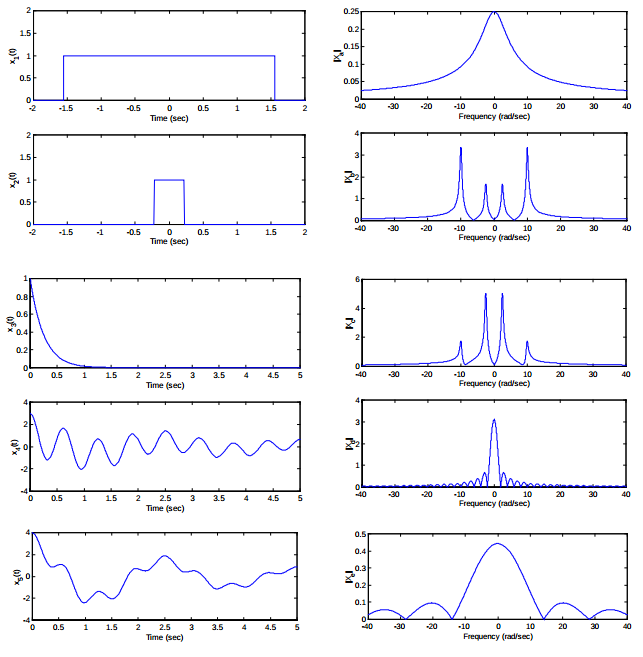
\includegraphics[width=0.8\textwidth]{figs/c2p7.png}
\label{fig:c2p7}
\end{figure} 

\subsection*{Solution}

As stated in (\ref{eq:c2p4}) the Fourier Transform of a Gate function is 
a Sa. The 1st gate is more spread in time that the 2nd and therefore
its corresponding transform must be more narrow. 

$1 \Leftrightarrow d $

$2 \Leftrightarrow e $

The 3rd plot corresponds to a negative exponential truncated by a step function.
We know for (\ref{eq:c2p5}) and for Points 6b and 6c that the corresponding 
transform corresponds to a figure like (a).

$3 \Leftrightarrow a $

From the following plots we see that the frecuency of 5 (rad/s) is more dominant
in the last one and the 10 (rad/s) is more dominant in the previous one.

$4 \Leftrightarrow b $

$5 \Leftrightarrow c $

